\documentclass[12pt,a4paper]{article}
%-------------------------------------------
%---Packages--------------------------------
%-------------------------------------------
\usepackage[utf8]{inputenc}
%\usepackage[T1]{fontenc}
%\usepackage{txfonts}
\usepackage{amsmath}
\usepackage{amsthm}
\usepackage{amsfonts}
\usepackage{array}
\usepackage{amssymb}
\usepackage{blindtext}
\usepackage{caption}
\usepackage{color}
\usepackage{csquotes}	    %
\usepackage{enumitem}	    %pour mieux bosser avec les listes. ajoute option label
\usepackage[yyyymmdd]{datetime}        %pour définir date custom
\usepackage{etaremune}
\usepackage{environ}
\usepackage{fancybox}
\usepackage{fancyhdr} 	    % Custom headers and footers
\usepackage{fancyref}
%\usepackage{float}
\usepackage{floatrow}       %float and floatrow can't be together...
\usepackage{gensymb}
\usepackage{graphicx}
\usepackage[colorlinks=true, linkcolor=purple, citecolor=cyan]{hyperref}
\usepackage{footnotebackref}
\usepackage{lipsum}
\usepackage{mathtools}
\usepackage{multicol}	    %gérer plusieurs colonnes
\usepackage{setspace}
\usepackage{subcaption}
\usepackage{todonotes}	    %Bonne gestion des TODOs
%TODO commenté pour tester l'utilité... à voir% \usepackage[tc]{titlepic}      %Permet de mettre une image en page de garde
\usepackage{tikz}	    % Pour outil de dessin puissant
\usepackage{ulem}	    %underline sur plusieurs lignes (avec \uline{})
\usepackage{vmargin} 	    %gestion des marges, avec dans l'ordre : gauche, haut, droit, bas, en-tête, entre en-tête et texte, bas de page, hauteur entre bas de page et texte
\usepackage{wrapfig}
\usepackage{xcolor}
\usepackage{xparse}                    %Pour utiliser NewDocumentCommand et des arguments 'mmooo'
%\usepackage{fullpage} 	    %supprime toutes les marges allouées aux notes, aussi en haut et en bas

%\ExplSyntaxOn
\pagestyle{fancyplain}	    %Makes all pages in the document conform to the custom headers and footers

%-------------------------------------------
%---Document Commands-----------------------
%---------------------------{----------------
\NewDocumentCommand{\framecolorbox}{oommm}
 {% #1 = width (optional)
  % #2 = inner alignment (optional)
  % #3 = frame color
  % #4 = background color
  % #5 = text
  \IfValueTF{#1}%
   {\IfValueTF{#2}%
    {\fcolorbox{#3}{#4}{\makebox[#1][#2]{#5}}}%
    {\fcolorbox{#3}{#4}{\makebox[#1]{#5}}}%
   }%
   {\fcolorbox{#3}{#4}{#5}}%
 }%
%------------------------------------------------
%------------------ENGLISH----------------------
%----------------------------------------------

\NewDocumentCommand{\epflTitle}{mO{Olivier Cloux}O{\today}O{Notes de Cours en}D<>{../../Common}}%Arguments : Matière, Auteur, Date, Titre du doc
{
\begin{titlepage}
    \vspace*{\fill}
    \begin{center}
        \normalfont \normalsize
        \textsc{Ecole Polytechnique Fédérale de Lausanne} \\ [25pt] % Your university, school and/or department name(s)
        \textsc{#4} %Titre du doc
        \\ [0.4 pt]
        \horrule{0.5pt} \\[0.4cm] % Thin top horizontal rule
        \huge #1 \\ % Matière
        \horrule{2pt} \\[0.5cm] % Thick bottom horizontal rule
        
\includegraphics[width=8cm]{#5/EPFL_logo}
        ~\\[0.5 cm]
        \small\textsc{#2}\\[0.4cm]
        \small\textsc{#3}\\
        ~\\
        ~\\
        
\includegraphics[scale=0.5]{#5/creativeCommons}
    \end{center}
    \vspace*{\fill}
\end{titlepage}
}


%-------------------------------------------
%-------------MATH NEW COMMANDS-------------
%-------------------------------------------
\newcommand{\somme}[2]{\ensuremath{\sum\limits_{#2}^{#1}}}
\newcommand{\produit}[2]{\ensuremath{\prod\limits_{#2}^{#1}}}
\newcommand{\limite}{\lim\limits_}
\newcommand{\llimite}[3]{\limite{\substack{#1 \\ #2}}\left(#3\right)}	%limites à deux condiitons
\newcommand{\et}{\mbox{ et }}
\newcommand{\deriv}[1]{\ensuremath{\, \mathrm d #1}}	%sigle dx, dt,dy... des dérivées/intégrales
%\newcommand{\fx}{\ensuremath{f'(\textbf{x}_0 + h}}
\newcommand{\ninf}{\ensuremath{n \to \infty}}	       %pour les limites : n tend vers l'infini
\newcommand{\xinf}{\ensuremath{x \to \infty}}	       %pour les limites : x tend vers l'infini
\newcommand{\infint}{\ensuremath{\int_{-\infty}^{\infty}}}
\newcommand{\xo}{\ensuremath{x \to 0}}									%x to 0
\newcommand{\no}{\ensuremath{n \to 0}}									%n zéro
\newcommand{\xx}{\ensuremath{x \to x}}									%x to x
\newcommand{\Xo}{\ensuremath{x_0}}										%x zéro
\newcommand{\X}{\ensuremath{\mathbf{X}} }
\newcommand{\A}{\ensuremath{\mathbf{A}} }
\newcommand{\R}{\ensuremath{\mathbb{R}} }								%ensemble de R
\newcommand{\rn}{\ensuremath{\mathbb{R}^n} } 							%ensemble de R de taille n
\newcommand{\Rm}{\ensuremath{\mathbb{R}^m} }  							%ensemble de R de taille m
\newcommand{\C}{\ensuremath{\mathbb{C}} }
\newcommand{\N}{\ensuremath{\mathbb{N}} }
\newcommand{\Z}{\ensuremath{\mathbb{Z}} }
\newcommand{\Q}{\ensuremath{\mathbb{Q}} }
\newcommand{\rtor}{\ensuremath{\R \to \R} }
\newcommand{\pour}{\mbox{ pour }}
\newcommand{\coss}[1]{\ensuremath{\cos\(#1\)}}						%cosinus avec des parenthèses de bonne taille (genre frac)
\newcommand{\sinn}[1]{\ensuremath{\sin\(#1\)}}					%sinus avec des parentèses de bonne taille (genre frac)
\newcommand{\txtfrac}[2]{\ensuremath{\frac{\text{#1}}{\text{#2}}}}		%Fractions composées de texte
\newcommand{\evalfrac}[3]{\ensuremath{\left.\frac{#1}{#2}\right|_{#3}}}
\renewcommand{\(}{\left(}												%Parenthèse gauche de taille adaptive
\renewcommand{\)}{\right)}
\newcommand{\longeq}{=\joinrel=}												%Parenthèse droite de taille adaptive


%-------------------------------------------------------
%------------------MISC NEW COMMANDS--------------------
%-------------------------------------------------------
\newcommand{\degre}{\ensuremath{^\circ}}
%\newdateformat{\eudate}{\THEYEAR-\twodigit{\THEMONTH}-\twodigit{\THEDAY}}



%-------------------------------------------------------
%------------------TEXT NEW COMMANDS--------------------
%-------------------------------------------------------
\newcommand{\ts}{\textsuperscript}
\newcommand{\evid}[1]{\textbf{\uline{#1}}}        %mise en évidence (gras + souligné)



%\newcommand{\Exemple}{\underline{Exemple}}
\newcommand{\Theoreme}{\underline{Théorème}}
\newcommand{\Remarque}{\underline{Remarque}}
\newcommand{\Definition}{\underline{Définition} }
\newcommand{\skinf}{\sum^{\infty}_{k=0}}
\newcommand{\combi}[2]{\ensuremath{\begin{pmatrix} #1 \\ #2 \end{pmatrix}}}	%combinaison parmi 1 de 2
\newcommand{\intx}[3]{\ensuremath{\int_{#1}^{#2} #3 \deriv{x}}}				%intégrale dx
\newcommand{\intt}[3]{\ensuremath{\int_{#1}^{#2} #3 \deriv{t}}}				%intégrale dy
\newcommand{\misenforme}{\begin{center} Mis en forme jusqu'ici\\ \line(1,0){400}\\ normalement juste, mais à améliorer depuis ici\end{center}}	%raccourci pour mise en forme
\newcommand*\circled[1]{\tikz[baseline=(char.base)]{
            \node[shape=circle,draw,inner sep=1pt] (char) {#1};}}			%pour entourer un chiffre
\newcommand{\horrule}[1]{\rule{\linewidth}{#1}} 				% Create horizontal rule command with 1 argument of height

\theoremstyle{definition}
\newtheorem{exemp}{Exemple}
\newtheorem{examp}{Example}


%-------------------------------------------
%---Environments----------------------------
%-------------------------------------------
\NewEnviron{boite}[1][0.9]{%
	\begin{center}
		\framecolorbox{red}{white}{%
			\begin{minipage}{#1\textwidth}
 	 			\BODY
			\end{minipage}
		}
	\end{center}
}
\NewEnviron{blackbox}[1][0.9]{%
	\begin{center}
		\framecolorbox{black}{white}{%
			\begin{minipage}{#1\textwidth}
 	 			\BODY
			\end{minipage}
		}
	\end{center}
}
\NewEnviron{exemple}[1][0.8]{%
    \begin{center}
        \framecolorbox{white}{gray!20}{%
            \begin{minipage}{#1\textwidth}
                \begin{exemp}
                    \BODY
                \end{exemp}
            \end{minipage}
        }
    \end{center}
}
\NewEnviron{suiteExemple}[1][0.8]{%
    \begin{center}
        \framecolorbox{white}{gray!20}{%
            \begin{minipage}{#1\textwidth}
                \BODY
            \end{minipage}
        }
    \end{center}
}
\NewEnviron{colExemple}[1][0.8]{%
    \begin{center}
        \framecolorbox{white}{gray!20}{%
            \begin{minipage}{#1\columnwidth}
                \begin{exemp}
                    \BODY
                \end{exemp}
            \end{minipage}
        }
    \end{center}
}
\NewEnviron{example}[1][0.8]{%
    \begin{center}
        \framecolorbox{white}{gray!20}{%
            \begin{minipage}{#1\textwidth}
                \begin{examp}
                    \BODY
                \end{examp}
            \end{minipage}
	}
    \end{center}
}
\NewEnviron{systeq}[1][l]{
			\begin{center}
				$\left\{\begin{array}{#1}
					\BODY
				\end{array}\right.$
			\end{center}
 }





%-------------------------------------------
%---General settings-----------------------
%-------------------------------------------
\renewcommand{\headrulewidth}{1pt}										%ligne au haut de chaque page
\renewcommand{\footrulewidth}{1pt}										%ligne au pied de chaque page
\setstretch{1.6}
\author{Olivier Cloux}

\usepackage{tikz}
\title{Série 1}
\date{}
\begin{document}
\maketitle
\part*{236079}
\evid{Problème 1.1}\\
\\
\begin{center}
\begin{tabular}{|c|c|c|c|c|c|c|}
m = & 1 & 2 & 3 & 4 & 5 & 6 \\
\hline
p(S = m) = &$\frac{1}{6}$&$\frac{1}{6}$&$\frac{1}{6}$&$\frac{1}{6}$&$\frac{1}{6}$&$\frac{1}{6}$\\
\end{tabular}\\\end{center}
${}$\\
\begin{enumerate}
	\item \underline{(1)} $P(E_1) = P(1) + P(3) + P(4) = \frac{1}{6} + \frac{1}{6} + \frac{1}{6} = \frac{3}{6} = $\fbox{$\frac{1}{2}$}\\
		\underline{(2)} $P(E_2) = P(3) + P(4) + P(5) + P(6) = \frac{4}{6} = $\fbox{$\frac{2}{3}$}.\\
		\underline{(3)} $P(E_3) = P(1) + P(2) = \frac{2}{6} =$ \fbox{$\frac{1}{3}$}.
	\item $E_1\cap E_2 = E_{1,2} = \{3,4\} \\
	\to P(E_1 \cap E_2) = P(E_{1,2}) = P(3) + P(4) = \frac{2}{6} =$ \fbox{$\frac{1}{3}$}.\\
	Avec la même idée : \\
	$E_1\cap E_3 = E_{1,3}  = \{1\}\to P(E_{1,3}) = P(1) =$ \fbox{$\frac{1}{6}$}.\\
	$E_2 \cap E_3 = E_{2,3} = \emptyset \to P(E_{2,3}) =$ \fbox{0}\\
	$E_1 \cap E_2 \cap E_3 = E_{2,3} \cap E_1 = E_{1,2,3} = \emptyset \to P(E_{1,2,3}) = P(E_{1,2}) =$ \fbox{0}
	\item $E_1 \cup E_2 = E_{1,2}' = \{1,3,4,5,6\} \to P(E_{1,2}') = $ \fbox{$\frac{5}{6}$}\\
	$E_1 \cup E_3 = E_{1,3}' = \{1,2,3,4\} \to P(E_{1,3}') = $ \fbox{$\frac{2}{3}$}\\
	$E_2 \cup E_3 = E_{2,3}' = \{1,2,3,4,5,6\} \to P(E_{2,3}') = \frac{6}{6} =$ \fbox{1}\\
	$E_1 \cup E_2 \cup E_3 = E_{2,3} \cup E_1 = \{1,2,3,4,5,6\} \to P(E_{1,2,3}') = P(E_{2,3}) =$ \fbox{1}
	\item Selon les lois d'indépendance d'un point de vue de probabilités, deux événements $E_i,E_j$ sont indépendants si et seulement si : $P(E_i \cap E_j) = P(E_i)\cdot P(E_j)$. Analysons ainsi deux à deux les couples possibles :
	\begin{itemize}
		\item $P(E_1\cap E_2) = \frac{1}{3} = \frac{1}{2}\cdot\frac{2}{3} = P(E_1)\cdot P(E_2) \to E_1$ et $E_2$ sont indépendants.
		\item $P(E_1 \cap E_3) = \frac{1}{6} = \frac{1}{2} \cdot \frac{1}{3} = P(E_1)\cdot P(E_2) \to E_1$ et $E_3$ sont indépendants.
		\item $P(E_2 \cap E_3) = 0 \neq\frac{2}{9} = \frac{2}{3} \cdot \frac{1}{3} = P(E_2)\cdot P(E_3) \to E_2$ et $E_3$ sont dépendants.
	\end{itemize}
		Comme nous venons de le voir, l'indépendance n'est pas transitive. En effet, $E_3$ et $E_1$ sont indépendants, $E_1$ et $E_2$ aussi, mais $E_2$ et $E_3$ sont dépendants.
\end{enumerate}
\evid{Problème 1.2}\\
\begin{enumerate}
	\item $H(S_1) = H(S_2)$, car les densités de probabilité sont les mêmes pour $x_{i1}$ et $x_{i2}$, les deux étant égaux. Leur entropie (selon la formule vue en cours) vaut :\\
	\underline{$H(S_1) = -q\log_2(q)-(1-q)\log_2(1-q) = H(S_2)$}\\
	\\
	Ce qui est alors étonnant, c'est que $H(S) = H(S_1) = H(S_2)$. En effet, une fois que $x_{i1}$ est tiré, on connaît directement $a_1$, ainsi, les densités de probabilité de $x_{i1}$ sont les mêmes que celles de $x_{i2}$, et donc de $a_i$\\
	$\to \underline{H(S) = H(S_1) = H(S_2) = -q\log_2(q)-(1-q)\log_2(1-q)}$\\
	Cela illustre le phénomène de dépendance. En effet, $H(S) < H(S_1) + H(S_2) = 2H(S)$. Cela montre très clairement que $S_1$ et $S_2$ sont dépendants (selon les lois d'entropie). En effet, la donnée précise que $S_1$ et $S_2$ sont \enquote{totalement} dépendants (en savoir un donne l'entièreté de l'information sur le second).\\
	\item Il est évident ici que $H(S_1)$ et $H(S_2)$ restent identique par rapport à l'exercice précédent. En effet, leur densité de probabilité ne change pas, donc leurs entropies non plus. En revanche, celle de S change, car connaître $S_1$ ne permet pas de déterminer $S$.\\
	S peut prendre 4 formes différentes possibles : \\
	(0,0), avec une probabilité $q^2$, \\
	(1,0) ou (0,1), chacun avec une probabilité $q(1-q)$\\
	(1,1), avec une probabilité $(1-q)^2$\\
	Ainsi, l'entropie de S vaut \\
	$\begin{array}{ll}
		H(S) &= -q^2\log_2(q^2) - 2q(1-q)\log_2\Big(q(1-q)\Big) -(1-q)^2\log_2\Big((1-q)^2\Big)\\
		& = -2q^2\log_2(q) -2q(1-q)\Big(\log_2(q)+\log_2(1-q)\Big) -2(1-q)^2\log_2(1-q)\\
		&= \log_2(q)\Big(-2q^2-2q(1-q)\Big) + \log_2(1-q)\Big(-2q(1-q)-2(1-q)^2\Big)\\
		&= -q\log_2(q)\Big(2q+2(1-q)\Big)-(1-q)\log_2(1-q)\Big(2q+2(1-q)\Big)\\
		&= 2\Big(\underbrace{-q\log_2(q) - (1-q)\log_2(1-q)}_{=H(S_1) = H(S_2)}\Big)\\
		&= H(S_1) + H(S_2)
	\end{array}$\\
	$\to H(S) = H(S_1) + H(S_2)$. \\
	Cela montre bien que $S_1$ et $S_2$ sont indépendants (par les lois d'entropie)
	\item Nous avons vu précédemment les probabilités d'apparition des couples (0,0), (0,1), (1,0), (1,1). Les probabilités d'apparition de $w$ et $z$ sont donc respectivement celles de (1,0) et (1,1) (également respectivement $q(1-q)$ et $(1-q)^2$). En revanche y peut s'obtenir soit avec (0,0), soit (0,1) (donc seulement si le premier tirage est 0). Cette probabilité est de $q^2 + q(1-q) = q\Big(q+(1-q)\Big) = q$.
	En résumé, la densité de probabilité est :
	\begin{tabular}{|c|c|c|}
	$w$  & $y$ & $z$	\\
		\hline
	$q(1-q)$ & $q$ & $(1-q)^2$ 
	\end{tabular}.\\
	L'entropie de cette source devient donc :\\
	$\begin{array}{ll}
	H(S_{wyz}) &= -q(1-q)\log_2\Big(q(1-q)\Big) - q\log_2(q) - (1-q)^2\log_2\Big((1-q)^2\Big)\\
	&= -q(1-q)\Big(\log_2(q) + \log_2(1-q)\Big) -q\log_2(q) - 2(1-q)^2\log_2(1-q)\\
	&= \log_2(q)\Big(-q(1-q)-q\Big) + \log_2(1-q)\Big(-q(1-q)-2(1-q)^2\Big)\\
	&= \log_2(q)\Big(-q + q^2 -q\Big) + \log_2(1-q)\Big(-q+q^2-2(1-2q+q^2)\Big)\\
	&= \log_2(q)(q^2-2q) + \log_2(1-q)(q^2-q-2+4q-2q^2)\\
	&= \log_2(q)(q^2-2q) + \log_2(1-q)(-q^2+3q-2)\\
	&=-q\log_2(q)(2-q) -(2-q)(1-q)\log_2(1-q)\\
	&= (2-q)\Big(\underbrace{-q\log_2(q) - (1-q)\log_2(1-q)}_{=H(S_1) \ = H(S_2)}\Big)\\
	&= 2H(S_1) -qH(S_1)\\
	&= H(S_1) + H(S_2) -qH(S_1)\\
	&= H(S) - qH(S_1)
	\end{array}$\\
	Sachant que $0\leq q\leq 1$ (règle élémentaire des probabilités), alors $H(S_{wyz}) \leq H(S) = H(S_1) + H(S_2)$. Cela s'explique par différentes raisons. Déjà, l'alphabet est réduit (de 4 à 3  \enquote{caractères}). Ensuite, connaître le premier tirage nous donnera beaucoup plus d'information sur la suite ; car si c'est un 0 qui sort en premier, alors il est garanti que $w$ sortira. Donc, nous avons besoin de moins d'informations pour pouvoir deviner l'issue du tirage, donc l'entropie s'en trouve diminuée d'autant.
\end{enumerate}
\evid{Problème 1.3}
\begin{enumerate}
	\item 
		\begin{enumerate}[label=(\alph*)]
		\item \underline{Oui, les deux lancers sont indépendants}. En effet, savoir le résultat du premier lancer ne nous permet pas de deviner le  second, ou au moins entrevoir un résultat. Chaque lancer sera aussi aléatoire que les précédents (car la pièce est standard entre autres).
		\item L'alphabet contient 2 \enquote{caractères} (\enquote{$P$} et \enquote{$F$}), chacun avec une probabilité de $\frac{1}{2}$. Selon notre cours, l'entropie d'une telle source vaut la somme négative des probabilités de chaque résultat multiplié par le logarithme en base 2 de cette même probabilité \\
			$\to H(S_1) = -p(P)\log_2(p(P)) - p(F)\log_2(p(F))$\\
			$= 0.5\log_2(2) + 0.5\log_2(2) = 1$. \underline{L'entropie de $S_1$ est donc d'un bit}. De plus, \underline{celle de $S_2$ vaut la même chose} (les conditions initiales et les probabilités sont les même, donc le calcul et le résultat sont aussi les mêmes). Enfin, sachant que $S_1$ et $S_2$ sont indépendants (voir 1.2(a)), l'entropie de $S$ vaut $S_1 + S_2 =$\underline{2 bits}
		\end{enumerate}
		\newpage
	\item ${}$
	\begin{enumerate}[label=(\alph*)]
		\item${}$
			\begin{center}
				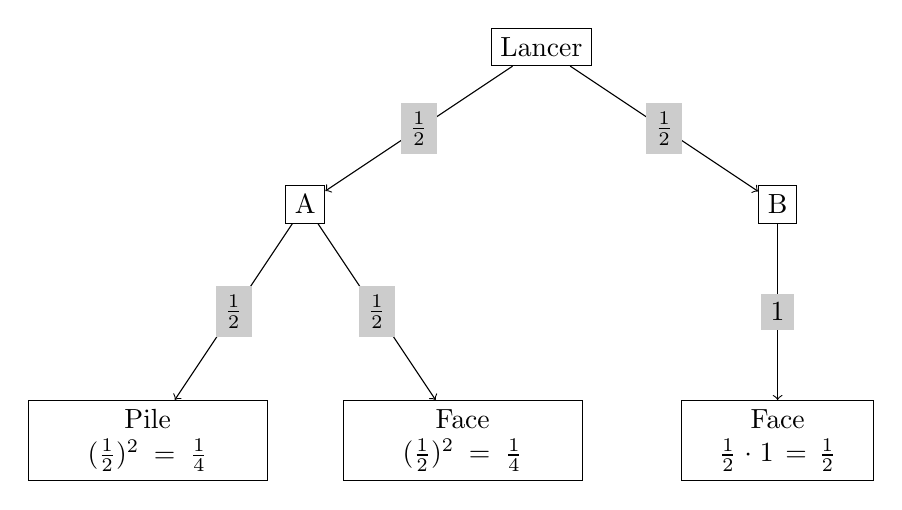
\begin{tikzpicture}
				\tikzstyle{etiquette}=[midway,fill=black!20]
				\node[draw] (L) at (0,0){Lancer};	
				\node[draw] (A) at (-3,-2){A};
				\node[draw] (B) at (3,-2){B};
				\node[draw, text width=2.8cm, text centered] (P) at (-5,-5){Pile \\ $(\frac{1}{2})^2 = \frac{1}{4}$};
				\node[draw, text width=2.8cm, text centered] (F1) at (-1,-5){Face \\ $(\frac{1}{2})^2 = \frac{1}{4}$};
				\node[draw, text width=2.2cm, text centered] (F2) at (3,-5){Face \\ $\frac{1}{2}\cdot 1 = \frac{1}{2}$};
				\draw[->] (L) -- (A)node[etiquette]{$\frac{1}{2}$};
				\draw[->] (L) -- (B)node[etiquette]{$\frac{1}{2}$};
				\draw[->] (A) -- (P)node[etiquette]{$\frac{1}{2}$};
				\draw[->] (A) -- (F1)node[etiquette]{$\frac{1}{2}$};
				\draw[->] (B) -- (F2)node[etiquette]{1};
			\end{tikzpicture}
		\end{center}
		Ainsi, Pile arrivera avec $\frac{1}{4}$, alors que Face arrivera avec\\ $\frac{1}{4} + \frac{1}{2} = \frac{3}{4}$
		\item${}$
					\begin{center}
				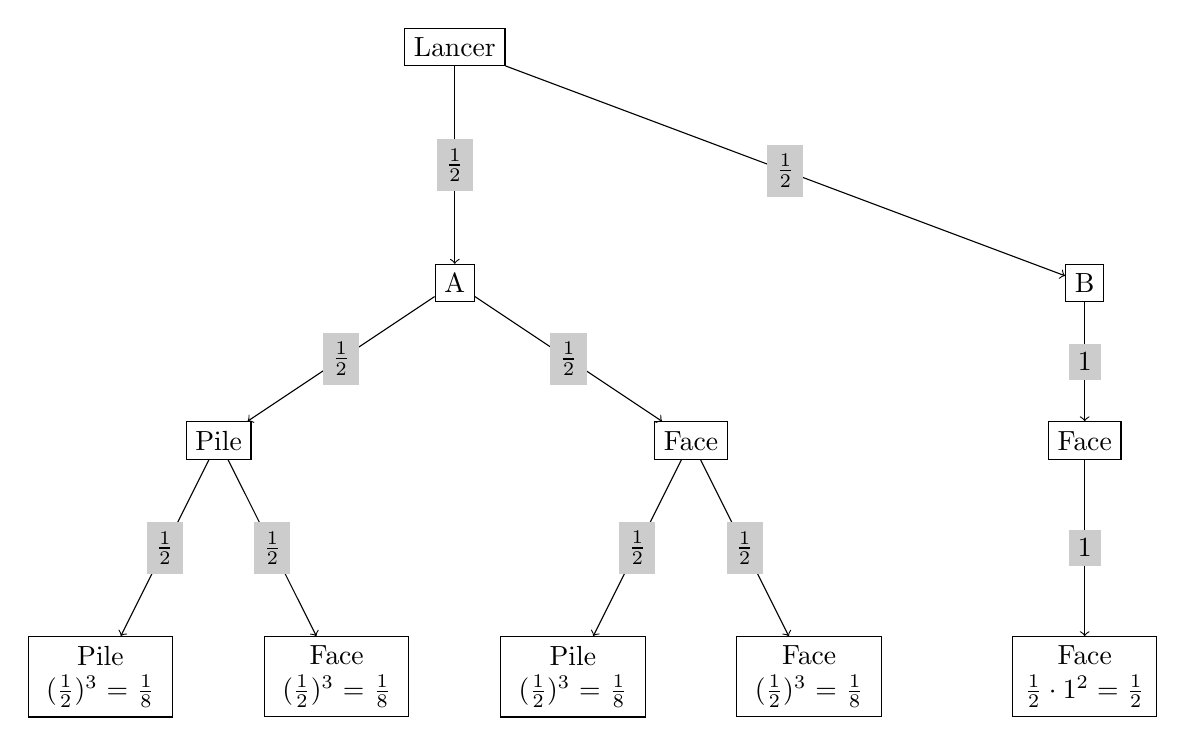
\begin{tikzpicture}
				\tikzstyle{etiquette}=[midway,fill=black!20]
				\node[draw] (L) at (-4,1){Lancer};	
				\node[draw] (A) at (-4,-2){A};
				\node[draw] (B) at (4,-2){B};
				\node[draw] (P11) at (-7,-4){Pile};
				\node[draw] (F11) at (-1,-4){Face};
				\node[draw] (F12) at (4,-4){Face};
				\node[draw, text width=1.6cm, text centered] (P21) at (-8.5,-7){Pile \\ $(\frac{1}{2})^3 = \frac{1}{8}$};
				\node[draw, text width=1.6cm, text centered] (F21) at (-5.5,-7){Face \\ $(\frac{1}{2})^3 = \frac{1}{8}$};			
				\node[draw, text width=1.6cm, text centered] (P22) at (-2.5,-7){Pile \\ $(\frac{1}{2})^3 = \frac{1}{8}$};
				\node[draw, text width=1.6cm, text centered] (F22) at (0.5,-7){Face \\ $(\frac{1}{2})^3 = \frac{1}{8}$};
				\node[draw, text width=1.6cm, text centered] (F23) at (4,-7){Face \\ $\frac{1}{2} \cdot 1^2 = \frac{1}{2}$};
				\draw[->] (L) -- (A)node[etiquette]{$\frac{1}{2}$};
				\draw[->] (L) -- (B)node[etiquette]{$\frac{1}{2}$};
				\draw[->] (A) -- (P11)node[etiquette]{$\frac{1}{2}$};
				\draw[->] (A) -- (F11)node[etiquette]{$\frac{1}{2}$};
				\draw[->] (B) -- (F12)node[etiquette]{1};
				\draw[->] (P11) -- (P21)node[etiquette]{$\frac{1}{2}$};
				\draw[->] (P11) -- (F21)node[etiquette]{$\frac{1}{2}$};
				\draw[->] (F11) -- (P22)node[etiquette]{$\frac{1}{2}$};
				\draw[->] (F11) -- (F22)node[etiquette]{$\frac{1}{2}$};
				\draw[->] (F12) -- (F23)node[etiquette]{1};
			\end{tikzpicture}
		\end{center}
		Nous voyons, grâce à l'arbre de probabilité ci-dessus, que : \\
		\fbox{$p(PP) = p(PF) = p(FP) = \frac{1}{8}$}\\
		et que\\
		 \fbox{$p(FF) = \frac{1}{8} + \frac{1}{2} = \frac{5}{8}$}
		\item Selon la formule de calcul de l'entropie vue en cours, et en ne considérant que $S_1$ (c.f. (a)).\\
		$\to H(S_1) = \frac{1}{4}\log_2(4) + \frac{3}{4}\log_2(\frac{4}{3}) \simeq$\fbox{0.811}\\
		L'entropie de $S_2$ est la même que celle que $S_1$ car nous n'avons pas encore regardé la pièce ; elle a donc toujours autant de chances d'être la pièce A que la B, et ainsi la densité de probabilité pour le second tire d'être pile ou face reste la même.\\
		$\to H(S_2) = H(S_1) \simeq$ \fbox{0.811}\\
		L'entropie de $S$ se calcule de la même manière, en considérant simplement l'alphabet et les densités de probabilités calculées en (b).\\
		$\to H(S) = \frac{1}{8}\log_2(8) + \frac{5}{8}\log_2(\frac{8}{5}) \simeq$ \fbox{1.548}
		\item Deux sources $S_1$ et $S_2$ sont indépendantes seulement si $H(S) (= H(S_1,S_2)) = H(S_1) + H(S_2)$.\\
		Or $H(S_1)+H(S_2) = 2\cdot H(S_1) \simeq 2\cdot 0.811 > 1.548 \simeq H(S)$. Ainsi, selon l'argument entropie, \underline{ces deux sources sont dépendantes}\\
		\\
		D'un point de vue de probabilités, deux sources sont indépendantes si et seulement si $p(S_1 = i$ et $S_2 = j) = p(S_1 = i)\cdot p(S_2=j)$ pour tout $i$ et $j$ dans les alphabets concernés. Nous considérons donc ici n'importe quelle couple, par exemple $S_1 = P$ et $S_2 = F$, mais le calcul fonctionne également pour n'importe quelle couple (PP, PF, FP ou FF).\\
		$p(S_1 = P$ et $S_2 = F) = p(PF) = \frac{1}{8}\footnote{c.f. (b)}\neq \frac{3}{16} = \frac{1}{4}\cdot\frac{3}{4} = p(S_1=P)\cdot p(S_2=F)$. Selon l'argument densité de probabilité, \\\underline{ces deux sources sont donc dépendantes}
		 
			\end{enumerate}
\end{enumerate}

\end{document}